%%%%%%%%%%%%%%%%%%%%%%%%%%%%%%%%%%%%%%%%%%%%%%
% Head matter - can we try to be consistent on
% included packages
\ifdefined\beamerclass
\else
    \def\beamerclass{beamer}
\fi
\documentclass[\beamerclass]{beamer}

\usepackage{pgfpages}
\mode<handout>{
  % \setbeamercolor{background canvas}{bg=black!20}
  \pgfpagesuselayout{2 on 1}[a4paper,border shrink=5mm]
}

%\documentclass{beamer}
\mode<presentation>
{\usetheme{default}
 \usecolortheme{default}
 \usefonttheme{default}
 \setbeamertemplate{navigation symbols}{}
 \setbeamertemplate{footline}[frame number]
% \setbeamertemplate{caption}[numbered]
 }
\usepackage[english]{babel}
\usepackage{algorithm}
\usepackage[noend]{algpseudocode}
\usepackage[utf8x]{inputenc}
\usepackage{graphicx}
\usepackage{hyperref}
%\graphicspath{{./images/}}
\usepackage{tikz}
\usetikzlibrary{shapes.geometric, arrows,chains}
\usepackage{booktabs,makecell,multirow,tabularx}
\usepackage{verbatim}
\renewcommand{\arraystretch}{1.2}
\renewcommand\theadfont{\normalfont\bfseries}
\usepackage{array}
\usepackage{listings}
\lstset{language=Java, showstringspaces=false}
\usepackage[normalem]{ulem}
\usepackage{bm}
\def\layersep{2.5cm}

\usepackage{xcolor}
%\usepackage{subfig}
\setbeamertemplate{caption}{\insertcaption}
\usepackage[caption=false]{subfig}
\usepackage{hyperref}
\usepackage{verbatim}
%\setbeamertemplate{caption}[numbered]%\numberwithin{figure}{section}
% Define block styles

\usetheme{Copenhagen}
\hypersetup{pdfstartview={Fit}}
\lstset{basicstyle=\small\ttfamily,breaklines=true}

\usepackage{xmpmulti}

\tikzstyle{decision} = [diamond, draw, fill=blue!20, 
    text width=4.5em, text badly centered, node distance=3cm, inner sep=0pt]
\tikzstyle{block} = [rectangle, draw, fill=blue!20, 
    text width=3em, text centered, rounded corners, minimum height=3em]
\tikzstyle{line} = [draw, -latex']
\tikzstyle{cloud} = [draw, ellipse, fill=red!20, node distance=3cm,
    minimum height=2em]
\tikzset{
  startstop/.style={
    rectangle, 
    rounded corners,
    minimum width=3cm, 
    minimum height=1cm,
    align=center, 
    draw=black, 
    fill=red!30
    },
  process/.style={
    rectangle, 
    minimum width=3cm, 
    minimum height=1cm, 
    align=center, 
    draw=black, 
    fill=blue!30
    },
  decision/.style={
    rectangle, 
    minimum width=3cm, 
    minimum height=1cm, align=center, 
    draw=black, 
    fill=green!30
    },
  arrow/.style={thick,->,>=stealth},
  dec/.style={
    ellipse, 
    align=center, 
    draw=black, 
    fill=green!30
    },
}
\tikzstyle{arrow} = [thick,->,>=stealth]

\tikzset{onslide/.code args={<#1>#2}{%
  \only<#1>{\pgfkeysalso{#2}} % \pgfkeysalso doesn't change the path
}}

\makeatletter
\newenvironment<>{btHighlight}[1][]
{\begin{onlyenv}#2\begingroup\tikzset{bt@Highlight@par/.style={#1}}\begin{lrbox}{\@tempboxa}}
{\end{lrbox}\bt@HL@box[bt@Highlight@par]{\@tempboxa}\endgroup\end{onlyenv}}

\newcommand<>\btHL[1][]{%
  \only#2{\begin{btHighlight}[#1]\bgroup\aftergroup\bt@HL@endenv}%
}
\def\bt@HL@endenv{%
  \end{btHighlight}%   
  \egroup
}
\newcommand{\bt@HL@box}[2][]{%
  \tikz[#1]{%
    \pgfpathrectangle{\pgfpoint{1pt}{0pt}}{\pgfpoint{\wd #2}{\ht #2}}%
    \pgfusepath{use as bounding box}%
    \node[anchor=base west, fill=orange!30,outer sep=0pt,inner xsep=1pt, inner ysep=0pt, rounded corners=3pt, minimum height=\ht\strutbox+1pt,#1]{\raisebox{1pt}{\strut}\strut\usebox{#2}};
  }%
}
\makeatother

\definecolor{darkblue}{RGB}{37,55,97}
\definecolor{mellowyellow}{RGB}{247,206,70}
\definecolor{almostwhite}{RGB}{254,255,255}
\definecolor{merrygreen}{RGB}{79,173,91}
\definecolor{funkyorange}{RGB}{240,154,56}

\addtobeamertemplate{footnote}{\hskip -2em}{}
\newcommand\blfootnote[1]{%
  \begingroup
  \renewcommand\thefootnote{}\footnote{#1}%
  \addtocounter{footnote}{-1}%
  \endgroup
}

\DeclareMathOperator{\softmax}{softmax}
\DeclareMathOperator{\ReLU}{ReLU}

%%%%%%%%%%%%%%%%%%%%%%%%%%%%%%%%%%%%%%%%%%%%%%
% Formatting for title page
\title[Auto-encoders]{Autoencoders and Self-supervised Learning}
\author{Jonathon Hare}
\institute[]
{
  Vision, Learning and Control\\
  University of Southampton 
}
\date{}
\subject{Computer Science}
\useoutertheme{infolines}
\setbeamertemplate{headline}{} %remove headline
\setbeamertemplate{navigation symbols}{} %remove navigation symbols
%%%%%%%%%%%%%%%%%%%%%%%%%%%%%%%%%%%%%%%%%%%%%%

\begin{document}

\begin{frame}[plain]
        \begin{tikzpicture}[overlay, remember picture, shift={(current page.south west)},font={\fontfamily{Montserrat-TOsF}\selectfont}]
        \fill [mellowyellow,text=almostwhite] (0,0) rectangle (\paperwidth, \paperheight);
        \draw (5.5,7) node [align=left,text=darkblue] {\Huge 
        \begin{tabular}{l} 
        \textbf{Learn}\\
        \textbf{Latent} \\
        \textbf{Representations} 
        \end{tabular}};
        \draw (11,1) node [align=left,text=darkblue] {\includegraphics[scale=0.15]{../vlc.png}};
        \end{tikzpicture}
\end{frame}

\begin{frame}
  \titlepage
\end{frame}
%-------------------------------------------------------------%
\begin{frame}
\frametitle{Low Dimensional Representations}

\begin{itemize}
  \item<+-> One of the common features of many of the deep learning models we have looked at to this point is that they often try to reduce the dimensionality of the input data in order to capture some kind of underlying information.
  \item<+-> In the last lecture this was particularly evident when when we looked at embedding models like word2vec which explictly try to capture relationships in the data in a low dimensional `latent' space.
\end{itemize}
\end{frame}

\begin{frame}
\frametitle{Self-supervised Learning}

\begin{figure}
  \centering
  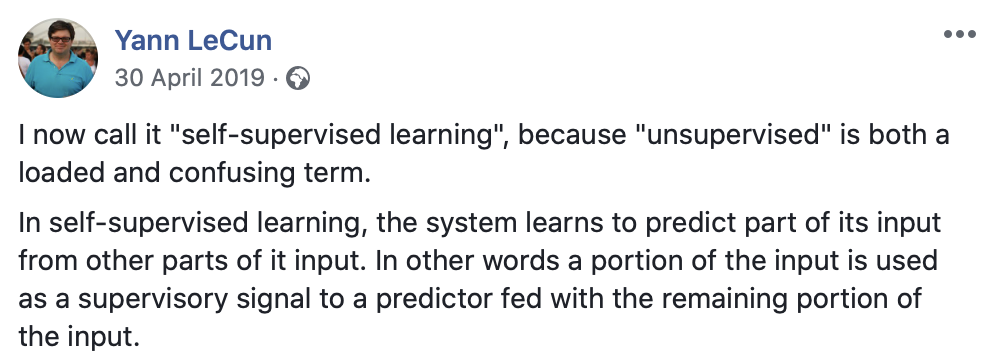
\includegraphics[width=\textwidth]{yann.png}
\end{figure}
\end{frame}

\begin{frame}
\frametitle{Self-supervised Learning}

\begin{itemize}
  \item<+-> The word2vec models are examples of \emph{self-supervised learning}
  \begin{itemize}
    \item<+-> CBOW learns to predict the focus word from the context words
    \item<+-> Skip-gram learns to predict the context words from the focus word
  \end{itemize}
  \item<+-> Let's now consider a different type self-supervised of task where we want to learn a model that learns to copy its input to its output.
\end{itemize}

\end{frame}

%-------------------------------------------------------------%
\begin{frame}
\frametitle{Autoencoders}

\begin{itemize}
  \item<+-> An \textbf{autoencoder} is a network that is trained to copy its input to its output
  \begin{itemize}
    \item<+-> Internally there is some hidden vector $\bm{h}$ that describes a \textbf{code} that represents the input.
    \item<+-> Conceptually the autoencoder consists of two parts:
    \begin{itemize}
      \item The encoder $\bm{h} = f(\bm{x})$
      \item The decoder $\bm{r} = g(\bm{h})$
    \end{itemize}
    \item<+-> and has loss that tries to minimise the reconstruction error (typically SSE/MSE: $\|\bm{x} - \bm{r}\|_2^2$)
  \end{itemize}
\end{itemize}
\begin{center}
\includegraphics<+->[width=5cm]{AE.pdf}
\end{center}
\end{frame}

\begin{frame}
\frametitle{Autoencoder constraints}

\begin{itemize}
  \item<+-> Clearly a linear autoencoder with a sufficient number of weights (e.g. if the dimension of $\bm{h}$ was greater than or equal to that of $x$) could learn set $g(f(\bm{x}))=\bm{x}$ everywhere, but this obviously wouldn't be useful!
  \item<+-> In practice we apply \emph{restrictions}\footnote{these are `inductive biases'} to stop this happening.
  \item<2-> The objective is to use these restrictions to force the autoencoder to learn useful properties of the data.
\end{itemize}

\end{frame}

\begin{frame}
\frametitle{Undercomplete Autoencoders}

\begin{itemize}
  \item Undercomplete autoencoders have $\dim(\bm{h}) << \dim(\bm{x})$.
  \item This forces the encoder to learn a \emph{compressed representation} of the input.
  \item The representation will capture the most \emph{salient} features of the input data.
\end{itemize}

\end{frame}


\begin{frame}{pause}
\frametitle{Undercomplete Autoencoders --- Linear}

Consider the single-hidden layer linear autoencoder network given by:

\begin{align*}
  h &= \bm{\mathrm{W}}_e \bm{x} + \bm{b}_e \\
  r &= \bm{\mathrm{W}}_d \bm{h} + \bm{b}_d
\end{align*}

where $\bm{x} \in \mathbb{R}^n$, $\bm{h} \in \mathbb{R}^m$ and $m<n$.\\[1em]
\pause
With the MSE loss, this autoencoder will learn to span the same subspace as PCA for a given set of training data. \\[1em]
Note that the autoencoder weights are not however constrained to be orthogonal (like they would be in PCA)
\end{frame}

\begin{frame}
\frametitle{Undercomplete Autoencoders --- deeper and nonlinear}

\begin{itemize}
  \item<+-> A linear autoencoder with a single hidden layer learns to map into the same subspace as PCA.
  \item<+-> Clearly, a deeper, linear autoencoder would also do the same thing.
  \item<+-> What happens if you introduce non-linearity?
  \begin{itemize}
    \item<+-> Interestingly, a single hidden layer network with non-linear activations on the encoder (keeping the decoder linear) and MSE loss also just learns to span the PCA subspace\footnote{Bourlard, H., Kamp, Y. Auto-association by multilayer perceptrons and singular value decomposition. Biol. Cybern. 59, 291–294 (1988). https://doi.org/10.1007/BF00332918}!
    \item<+-> But, if you add more hidden layers with non-linear activations (to either the encoder, decoder or both) you can effectively perform a powerful non-linear generalisation of PCA
  \end{itemize}
\end{itemize}
\end{frame}

\begin{frame}
\frametitle{Deep Autoencoders}
\begin{center}
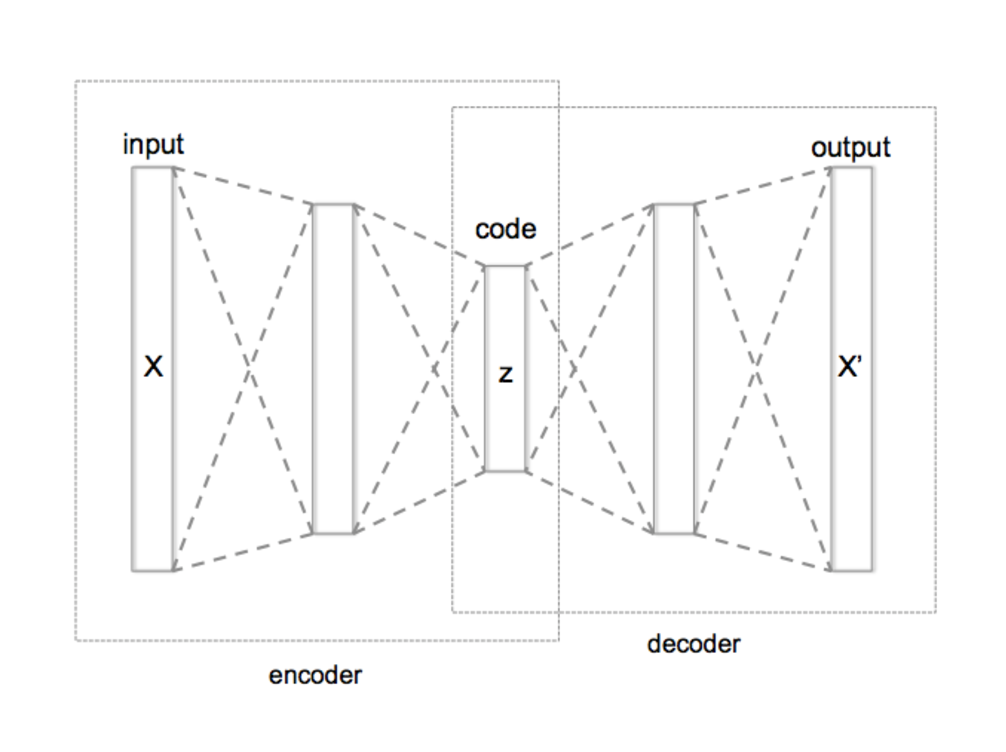
\includegraphics[width=10cm]{DAE.pdf} \blfootnote{Image taken from wikipedia}
\end{center}
\end{frame}

\begin{frame}
\frametitle{Deep Autoencoders - caveat}

\begin{itemize}
  \item<+-> There is a slight catch: if you give the deep autoencoder network too much capacity (too many weights) it will learn to perform the copying task without extracting anything useful about the data.
  \item<+-> Of course this means that will likely not generalise to unseen data.
\end{itemize}

\begin{itemize}
  \item<+-> Extreme example: 
  \begin{itemize}
    \item<+-> Consider a powerful encoder that maps $\bm{x}$ to $\bm{h} \in \mathbb{R}^1$
    \item<+-> Each training example $\bm{x}^{(i)}$ could e.g. be mapped to $i$.
    \item<+-> The decoder just needs to memorise the training examples so that it can map back from $i$.
  \end{itemize}
\end{itemize}
\end{frame}

%-------------------------------------------------------------%

\begin{frame}
\frametitle{Undercomplete Autoencoders --- Convolutional}
\begin{itemize}
\item<+-> Thus far, we only considered autoencoders with vector inputs/outputs and fully-connected layers.
\item<1-> There is nothing stopping us using any other kinds of layers though...
\item<2-> If we're working with image data, where we know that much of the structure is `local', then using convolutions in both the decoder makes sense
\end{itemize}
\end{frame}

\begin{frame}
\frametitle{Convolutional Autoencoder}


\end{frame}

%-------------------------------------------------------------%

\begin{frame}
\frametitle{Regularised Autoencoders}

\begin{itemize}
  \item<+-> Rather than (necessarily) forcing the hidden vector to have a lower dimensionality than the input, we could instead utilise some form of regularisation to force the network to learn interesting representations...
  \item<+-> Many ways to do this; let's look at two of them:
  \begin{itemize}
    \item Denoising Autoencoders
    \item Sparse Autoencoders
  \end{itemize}
\end{itemize}

\end{frame}

%-------------------------------------------------------------%

\begin{frame}
\frametitle{Denoising Autoencoders}

\begin{itemize}
\item<+-> Denoising autoencoders take a partially corrupted input and train to recover the original undistorted input.
\item<+-> To train an autoencoder to denoise data, it is necessary to perform a preliminary stochastic mapping to corrupt the data ($x \rightarrow \tilde x$). 
\begin{itemize}
  \item E.g. by adding Gaussian noise.
\end{itemize}
\item<+-> The loss is computed between the reconstruction (computed from the noisy input) against the original noise-free data.
\end{itemize}
\end{frame}

%-------------------------------------------------------------%

\begin{frame}
\frametitle{Sparse Autoencoders}

\begin{itemize}
\item<+-> In a sparse autoencoder, there can be more hidden units than inputs, but only a small number of the hidden units are allowed to be active at the same time.
\item<+-> This is simply achieved with a regularised loss function: $\ell = \ell_{mse} + \Omega(\bm{h})$
\item<+-> A popular choice that you've seen before would be to use an l1 penalty $\Omega(\bm{h} = \lambda \sum_i | h_i |$
  \begin{itemize}
    \item<+-> this of course does have a slight problem... what is the derivative of $y=|x|$ with respect to $x$ at $x=0$?
  \end{itemize}
\end{itemize}
\end{frame}

%-------------------------------------------------------------%

\begin{frame}\frametitle{Autoencoder Applications}
\begin{itemize}
\item<+-> Any basic AE (or its variant) can be used to learn a compact representation of data.
\begin{itemize}
  \item<+-> You can learn useful features from data without the need for labelled data.
  \item<+-> Denoising can help generalise over the test set since the data is distorted by adding noise.
\end{itemize}
\item<+-> Pretraining networks
\item<+-> Anomoly Detection
\item<+-> Machine translation
\item<+-> Semantic segmentation
\end{itemize}
\end{frame}

%-------------------------------------------------------------%
\begin{frame}
\frametitle{Beyond Deterministic Autoencoders: Stochastic Encoders and Decoders}
\begin{itemize}
\item<+-> When we trained supervised classification networks we usually assume that the network produces an output distribution $p(\bm{y}|\bm{x})$ and try to minimise the log-likelihood $-\log(p\bm{y}|\bm{x})$.
\item<+-> In a decoder of an autoencoder we could do the same thing and have the decoder learn $p_{decoder}(\bm{x}|\bm{h})$  by minimising $-\log(p\bm{x}|\bm{h})$.
\begin{itemize}
  \item<+-> A linear output layer could parameterise the mean of a Gaussian distribution for real-valued $\bm{x}$; in this case the negative log likelihood yields the MSE criterion.
  \item<+-> Binary $\bm{x}$ would correspond to a Bernoulli distribution parameterised by sigmoid outputs
  \item<+-> Discrete (or categorical) $\bm{x}$ would correspond to a softmax distribution.
\end{itemize}
\item<+-> What about the encoder - could we make that output $p(\bm{h} | \bm{x})$?
\end{itemize}
\end{frame}
%-------------------------------------------------------------%

\end{document}